\chapter{INTRODUCTION}

% \pagestyle{plain}

\label{introduction}

\section{Common formatting problems when using \LaTeX \ to write the dissertation.}
\begin{enumerate}
	\item The most common formatting problem is that the bottom margin of all pages is not between 1.25 and 1.5 inches.  The left and right margins are not between 1.25 and 1.5 inches.  This is true regardless of whether you are using LaTeX on Linux or Windows.
	\\
	Solution:  The problem with this is that dvipdf defaults to a paper size of A4, which is longer and narrower than 8.5" by 11".  This affects the left, right, and bottom margins.  To produce a document with the correct dimensions, in Linux first generate the DVI file.  Convert this file to postscript, then convert the postscript file to PDF using the following two commands:
	\begin{verbatim}
        dvips -t letter -Ppdf -G0 utaexample.dvi
        ps2pdf utaexample.ps
	\end{verbatim}	
    If you are using LaTeX on Windows, you may (depending on how your 
    environment is configured) be able to open a command window and
    type 
	\begin{verbatim}
       dvips -t letter -Ppdf -G0 utaexample.dvi
       ps2pdf utaexample.ps
	\end{verbatim}	
    to generate a PDF with the correct dimensions.
	\item Titles in the front matter and text longer than one line are appearing double-spaced in the front matter, but they should be single spaced.
	\\
	Solution: The sample document included with the template show examples of this and how to correct them.  Basically, at the point where you have the section title, caption title, etc., you need to create two versions of it.  One version will appear at that location in the document, the other version will appear in the table of contents and will include formatting commands specifically for the table of contents.  YOU DO NOT HAVE TO CHANGE THE TEMPLATE ITSELF FOR THIS PROBLEM.
\end{enumerate}


\section{Introduction}
% no \PARstart
Mobile station (MS) needs to maintain a target $E_b/N_0$ in a
power-controlled CDMA system to achieve the required frame error
rate. The fraction of base station (BS) power required by the MS
to maintain the target $E_b/N_0$ is different when the MS is in
different operation mode. When the MS is connected to multiple
BSs, it is said to be in soft handoff mode (SHM). While the MS is
only connected to a single BS, it is said to be in non-soft
handoff mode (NSHM). The MS in SHM achieves the macrodiversity
gain and decreases the power required from the base stations that
it is connected to. Current literature usually models $E_b/N_0$ as
a random variable to calculate outage probability and capacity
[1]. However, the $E_b/N_0$ is actually a constant value (or a
small range of value) from the power-control viewpoint. When
$E_b/N_0$ at the MS is less than the target value, the MS asks BSs
to increase the transmitted power. When the fraction of BS power
required by MS exceeds the maximum threshold, MS would not be able
to maintain target $E_b/N_0$, which could lead to the dropout of
the connections. Therefore, it is more appropriate to evaluate the
system performance from the viewpoint of the fraction of BS power
allocated to the MS.

Different approaches exist in the literatures to classify the MS
to be in SHM or NSHM. Lee and Steel [1] proposed the concept of
soft handoff zone (SHZ) and non-soft handoff zone (NSHZ). The NSHZ
is the area around the reference BS within radius less than a
certain distance $R_h$. The MS in NSHZ is only connected to the
reference BS regardless of the signal strengths received from
other BSs. The SHZ is the area around the reference BS with radius
greater than $R_h$ but less than the cell radius $R$. The MS in
SHZ utilizes all the received signals from the surrounding BSs.
The location of the boundary of SHZ and NSHZ is determined by the
pilot strength between two BSs and the shadowing effect is
ignored. $R_h$ is chosen to be $0.84R$. This approach was adopted
in a large number of literatures [1] . By putting the MS in SHZ
and NSHZ, the problem of soft handoff becomes simpler. However,
there are unconvincing disadvantages of the above approach. First,
explicit classification of SHZ and NSHZ does not exist in
practical CDMA systems. As the MS in SHZ can still maintain the
target $E_b/N_0$ by only connected to the reference BS and vice
versa. Second, the $R_h$ can not be explicitly defined by only the
path loss without considering the shadowing effects. As shadowing
fading exists, the MS in NSHZ may need to connect to multiple BSs
to maintain the target $E_b/N_0$ and vice versa. Therefore, it is
more accurate to define SH and NSH by considering the path loss
including the shadowing effect and considering NSH for the MS in
SHZ and SH for the MS in NSHZ. In this paper, we propose to use
the relative soft handoff threshold to classify the MSs in SHM and
NSHM. Using this approach, the BSs that the MS is connected to is
determined by the path loss difference from that of a reference
BS, where the reference BS has the lowest path loss (or the
strongest signal). The path loss difference is the soft handoff
threshold (SHT). Using that model, the MS in the SHZ can be in SH
with other BSs with a certain probability.

Using the proposed soft handoff model and assuming the Rake
receiver at the MS use channel-gain-and-interference matched
approach to combine the recevied signals from different BSs
.
We further simplify the expression of $E_b/N_0$ into one term and
derive the probability density function (PDF) of the fraction of
BS power allocted to the MS. By imposing an upper limit on the
maximum fraction of BS power (MFBP) allocated to the MS, the
capacity and outgage probability is derived analytically. We show
that the location of SH boundary, which is defiend at the
limitation of the system capacity, is
determined by the MFBP and SHT. We further show that contradict to
what commonly believed in previous literatures,
the SH can provide capacity gain only at a larger MFBP and SHT. SH
in this case only has the advantage of reducing the outage
probability.

This paper is organized as follows. Section II discusses the
system model and how to use path loss with shadowing and relative
soft handoff threshold to classify the MS in SHM or NSHM. Section
III shows the derivation of the distribution of the BS power. The
analytical derivation of the capacity and outage probability are
also presented in this section. Section IV gives the numerical
results and shows how the MFBP and SHT affect capacity and outage.
Section V summarizes the results.

\section{System model}
In our analysis, a 13 cells cluster is considered and shown in
Fig. \ref{figrawcon:1} in order to minimize edge effect, which is
caused if the BSs surrounding the MS is not symmetric. Only MSs
inside the triangle shown in Fig. \ref{figrawcon:1} are
considered. Due to the symmetry in the structure, the performance
matrix of the system obtained in this triangle can be generalized
to the whole reference cell.
\begin{figure}[tbp]
 \centerline{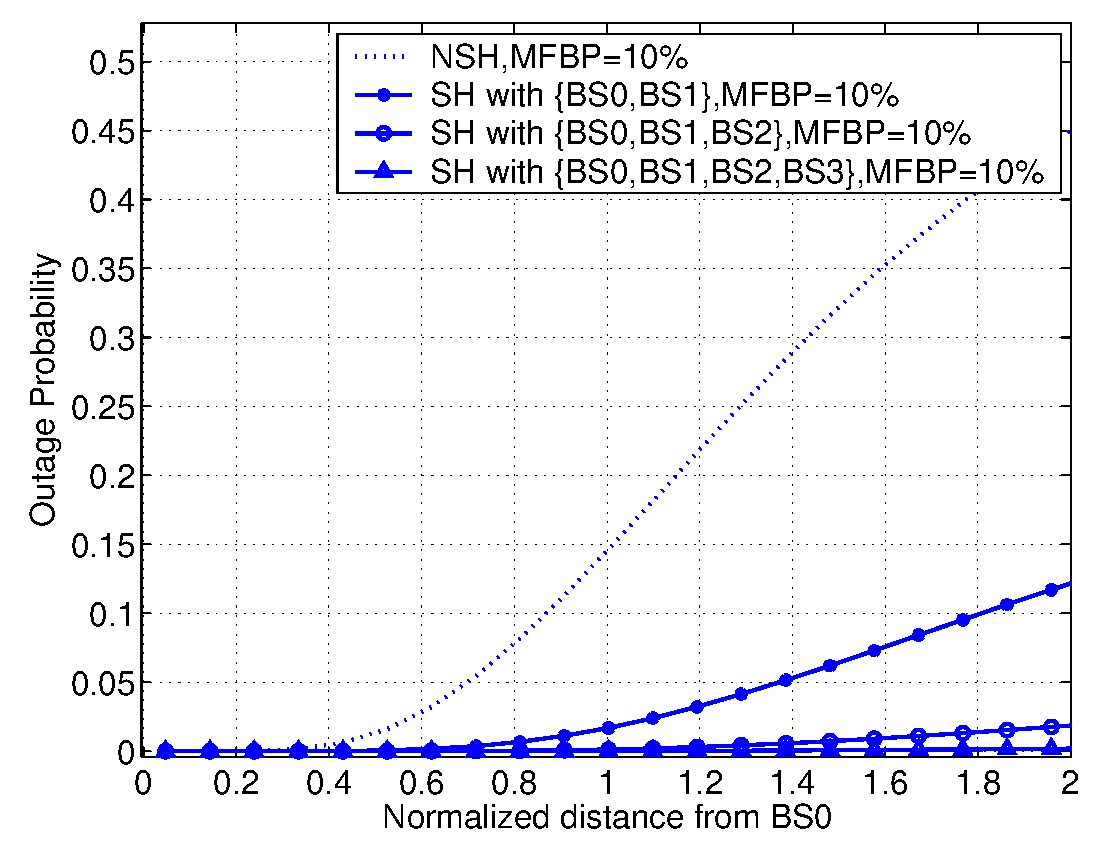
\includegraphics[width=3in,height=2.7in]{./separateoutage10.eps}}
 \caption{Cell structure} \label{figrawcon:1}
\end{figure}

\subsection{Soft Handoff Model}
\label{shdefinition} The SH approach used in the industry is
complex to analyze.

\begin{table}[htbp]

  \centering

  \caption{Base Class 0 System Frequecies}

\begin{tabular}{|c|c|c|}

\hline

System&Reverse Link (MHz)& Forward Link (MHz)\\

\hline

A&824-835&869-880 \\

&845-846.5 & 890-891.5 \\

\hline

B&835-845&880-890 \\

&846.5-849&891.5-894 \\

\hline

\end{tabular}

  \label{tableintro:1}

\end{table}

For example, IS-95 uses fixed or constant $T_{ADD}$, $T_{DROP}$
handoff thresholds and a $T_{TDROP}$ timer to choose the BSs in
the active set, which is defined as the set of BSs that the MS is
communicating with and requiring power from. When the estimated
pilot signal strength from a certain BS is above $T_{ADD}$, that
BS is put into the active set. The MS combines signals from up to
two BSs in the active set and having stronger pilot strengths. If
pilot signal strength BSs in active sets drops below $T_{DROP}$
for at least $T_{TDROP}$ time, the BS is taken away from the
active set [1]. The signal strength in IS-95 is defined as the
energy-per-chip-to-interference ratio of the pilot channel.
However, we can define pilot signal strength as the inverse of
path loss with shadowing to effectively classify the MS into NSHM
and SHM for the following reasons: First, the active set should be
designed to be as stable as possible, which means the fast fading
(also called as the small-scale fading [1]) had better be excluded
from the choice of the active set. For example, the pilots in
IS-95 are sent every 26.66ms for a spread rate of 1.2288Mcps
\footnote{chip per second} and there are enough fast fading
samples to be averaged out in the choice of the active set
\footnote{The fast fading samples have correlation coefficients
greater than zero for a duration of about 4ms at doppler shift of
100Hz [1]}. Therefore, the selection of the active set had better
be determined by the path loss with the slow varying shadowing
effect. Second, in practical CDMA systems (For example, IS-95),
the MS can easily estimate the time delay, the phase and magnitude
of the multipath components to find the stronger signal components
[1]. This is because the pilot channel signal level is 4 to 6 dB
higher than the traffic channel and the interference mainly comes
from pilot channels from surrounding BSs. Third, the usage of
$T_{TDROP}$ timer to model the duration of BSs in the active set
can be ignored in the system level design. $T_{TDROP}$ is useful
to account for the the correlation between signals in adjacent
locations (or time interval) and avoids unnecessary handoff
traffic. However, in system level design, the area taken into
consideration is large enough and in the order of 10m. Therefore,
the fadings between different location areas are independent [1].
Finally, the estimation of the pilot signal strength in term of
path loss with shadowing is as easy as the estimation of
energy-per-chip-to-interference. Lognormal distributed large-scale
shadowing path loss model [1] is more appropriate to select BS
into the active set.

This approach is established as follows: First, if we assume that
the fraction of BS power allocated from different BSs to MS are
the same in the forward link of a power-controlled system, we can
use normalized path loss to define reference BS$_{0}$ as the one
having the smallest path loss as shown in Fig. \ref{figrawcon:2}.
Second, if the path loss of a BS exceeds that of the reference
BS$_0$ by less than Th dB, that BS is put in the active set (or in
soft handoff with the MS). If the path loss of a BS exceeds that
of the reference BS$_0$ by greater than Th dB, that BS is not in
the active set (or in non-soft handoff with the MS). Third, if
other BS has path loss less than the current reference BS$_{0}$,
the reference BS is changed to that BS. The MS always connects to
the BSs in the active set and the active set always includes the
reference BS.

The definition of reference BS has its meanings in the reverse
link. Because the reference BS has the lowest path loss
\footnote{The path loss is the mean (local mean or time average)
path loss and takes into account of the large-scale lognormal
shadowing, which is the shadowing effects due to blocking between
the transmitter and the receiver} and due to the symmetric of
propagation [1], the signal received at the reference BS from the
MS is the strongest and more likely has a lower average frame
error rate (FER) \footnote{FER is determined by the
signal-to-interference ratio at the BS. However, the interference
level can be assumed to be the same if assuming all BSs are
equally loaded and the MSs is uniformly distributed in every
cell.}. The reverse link uses the select combination to select the
BS having the smallest FER [1] to power-control the MS and
thereby, the reference BS is more likely to be the power-control
BS for the MS in the reverse link.
\begin{figure}[tbp]
 \centerline{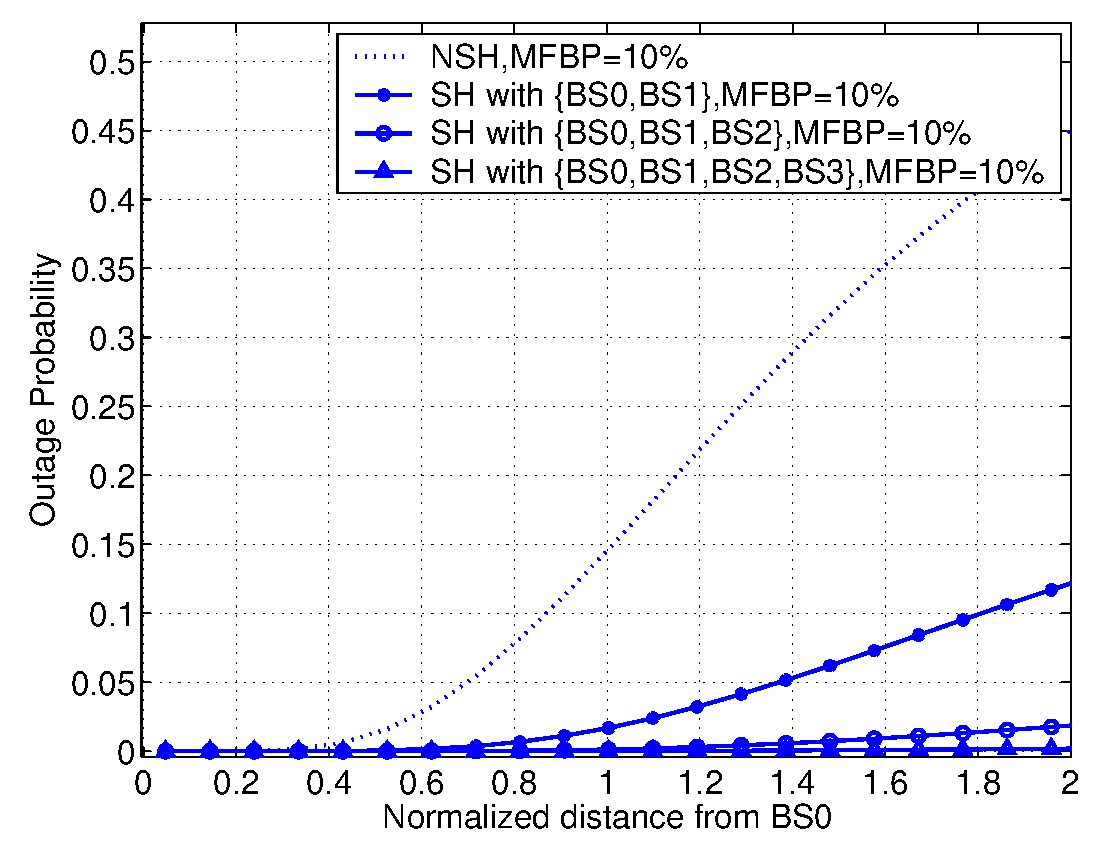
\includegraphics[width=3.5in,height=1.5in]{./separateoutage10.eps}}
 \caption{Soft handoff model using relative pilot strengths} \label{figrawcon:2}
\end{figure}

%\subsection[Path Loss Model That Is So Important That The\protect \vspace{-2ex} \\Subsection Title Can't Fit Onto A Single Line]{Path Loss Model That Is So Important That The Subsection Title Can't Fit Onto A Single Line}
%\subsection[Path Loss Model That Is So Important That The\protect \vspace{-2ex} \\Subsection Title Can't Fit Onto A Single Line\protect \vspace{-2ex} \\and Requires Three Lines to Display]
\subsection[This is an example of a very long section title.  It should\protect \vspace{-2ex}\\ appear single-spaced in the table of contents and not
\protect \vspace{-2ex} \\ extend all the way to the page numbers.  Look in the\protect \vspace{-2ex} \\file chap1.tex to see how this is done.]
{This is an example of a very long section title.  It should appear single-spaced in the table of contents and not extend all the way to the page numbers.  Look in the file chap1.tex to see how this is done.}
Symmetric correlated lognormal shadowing model is a simple but
effective approach to study the correlation between received
signals from different BSs. This model was adopted widely [1]. The
path loss $l_i$ from BS$_{i}$ to the MS is assumed to follow a
lognormal distribution and is expressed as $l_i = r_i^u 10^{x_i /
10}$, where r$_{i}$ is normalized distance from BS$_{i}$ to the MS
(normalized to the radius of the cell), $u$ is path loss slope and
x$_{i}$ is a Gaussian random variable with zero mean and $\sigma$
standard deviation. Usually, the path loss can be expressed in dB
as
\begin{equation}
\label{eqrawcon:1} L_i=10\log _{10} l_i = 10\log _{10} (r_i^u
10^{x_i / 10}) = M_i + a\xi + b\xi _i
\end{equation}

\noindent where $M_i = 10u\log _{10} (r_i )$ and x$_{i }$ is
expressed as the weighed summation of two independent Gaussian
random variables $\xi$ and $\xi_i$ with identical zero mean and
$\sigma$ standard deviation to account for correlation effects.
Signals from different BSs are assumed to have the same
correlation coefficient of $E[x_i x_j ] / \sigma ^2 = a^2$, $i \ne
j$ if we limit $a^2 + b^2 = 1$.

\subsection{Soft handoff and Non-soft Handoff Probability}
\label{sec:sh} Assume the active set is
$N_{set}=\{0,i_{1},i_{2},...,i_{M}\}, i_{k}\in \{1,2,\ldots ,N\}$,
where $N$ is the total number of BSs taken into consideration
(refer to Fig. \ref{figrawcon:1}, $N$ is 13 in our cells cluster
structure). Following the definition of the SH and NSH in section
\ref{shdefinition}, the probability of SH with active set
$N_{set}$ is derived as

\begin{equation}
\label{eqrawcon:3}\begin{split}
P\{NSH\}=&P\{L_0 + Th < L_i,i=1,2,\cdots,N\} \\
=& E_z[\prod\limits_{i = 1}^{N} Q(z + c_i )]
\end{split}
\end{equation}















%  vkp
